\hspace{0.5cm} Our proposed algorithm is first to implement \cite{bib11} which formulates style transfer as an image reconstruction process coupled with feature transformation,
i.e., whitening and coloring. The reconstruction part is responsible for inverting features back to the
RGB space and the feature transformation matches the statistics of a content image to a style image.
We used a pre-trained weights which was trained by VGG-19 \cite{bib20} encoder using ImageNet dataset (Deng et al.) \cite{bib21}.
Second, we show an improved algorithm which merges two style images bu using WCT algorithm which based on singular value decomposition (SVD). Here, we both implement the original merge algorithm as proposed in \cite{bib11} as well as introduce three additional efficient methods based on the use WCT.
\begin{figure}[h!]
	\centering
		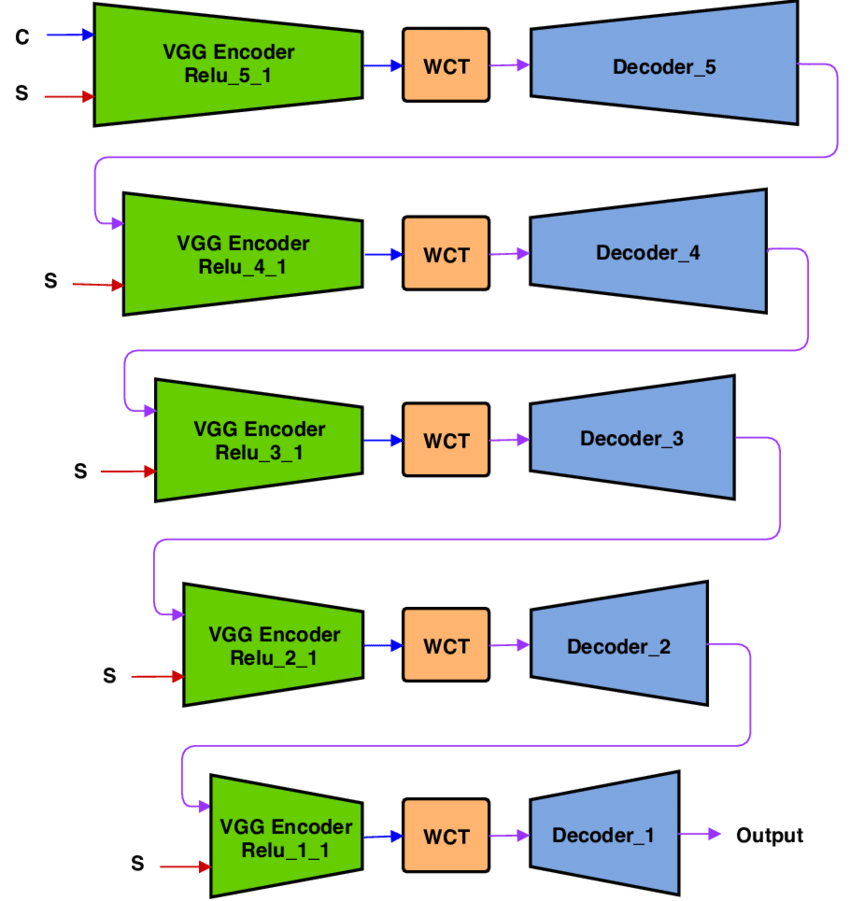
\includegraphics[width=0.5\linewidth]{UST_arc_mlt_level_pipeline.png}
	\caption{Universal Style Transfer architecture with the whole multi level pipeline. Each level of stylization consists of single encoder-WCT-decoder network with different decreasing number of VGG layers. C and S are content and style images, respectively.
	}
	\label{fig:full-pipeline}
\end{figure}
%%%%% 3.1 stylization %%%%%
\newline
\newline\textbf{3.1  Stylization}\newline
\newline \textbf{WCT}. The WCT \cite{bib11} formulates stylization as an image reconstruction problem with feature projections. To utilize WCT, an auto-encoder for general image reconstruction is first trained. We used the VGG-19 model \cite{bib20} as the encoder $\varepsilon$(weights are kept fixed) and trains a decoder D for reconstructing the input image. The decoder is symmetrical to the encoder and uses up-sampling layers to enlarge the spatial resolutions of the feature maps, (see figure ~\ref{fig:full-pipeline}). Once the auto-encoder is trained, a pair of projection functions are inserted at the network bottleneck to perform stylization through the whitening ($P_C$) and coloring ($P_S$) transforms. The key idea behind the WCT is to directly match feature correlations of the content image to those of the style image via the two projections. Specifically, given a pair of content image $I_C$ and style image $I_S$, the WCT first extracts their vectorised VGG features $C_f=\varepsilon(I_C)$ and $S_f=\varepsilon(I_S)$, and then transform the content feature $C_f$ via
\begin{equation}
CS_f = P_SP_CH_C
\end{equation}
Where $P_C=E_C\Lambda_C^{-\frac{1}{2}}$, and $P_S=E_S\Lambda_S^{\frac{1}{2}}$. Here $\Lambda_C$ and $\Lambda_S$ are the diagonal matrices with the eigenvalues of the covariance matrix $C_fC_f^T$ and $S_fS_f^T$ respectively. The matrices $E_C$ and $E_S$ are the corresponding orthonormal matrices of the eigenvalues, respectively, (see figure ~\ref{fig:WCT}). After the transformation, the correlations of
transformed features match those of the style features, i.e., $CS_fCS_f^T=S_fS_f^T$. Finally, the stylized image is obtained by directly feeding the transformed feature
map into the decoder: $Y = D(CS_f)$. For better stylization performance, Li et
al. \cite{bib11} use a multi-level stylization strategy, which performs the WCT on the
VGG features at different layers.
The WCT performs well for artistic image stylization. However it generates
structural artifacts (e.g., distortions on object boundaries)
%%% whitening-coloring figures %%%
\begin{figure}[h!]
	\centering
	\begin{subfigure}[b]{0.4\linewidth}
	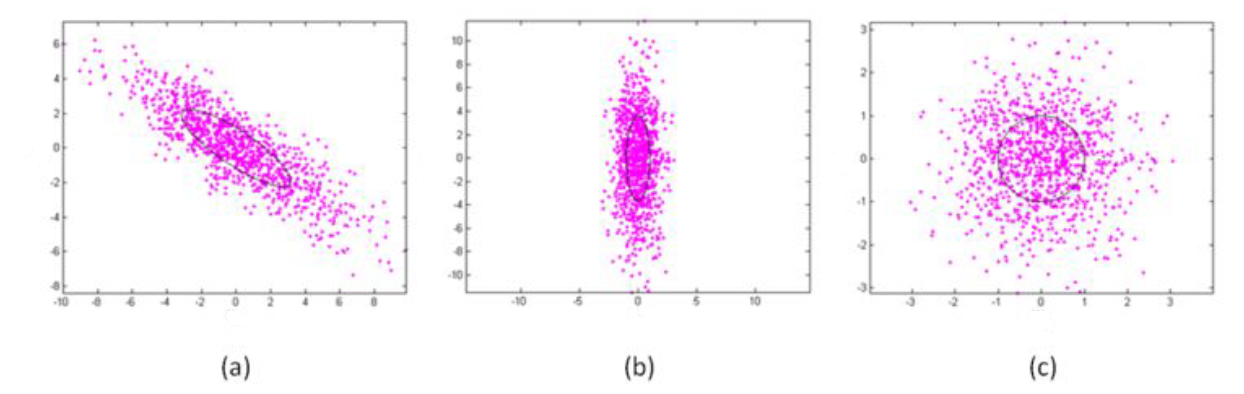
\includegraphics[width=\linewidth]{whitening.png}
		\caption{Data whitening}
		\end{subfigure}
	\begin{subfigure}[b]{0.4\linewidth}
	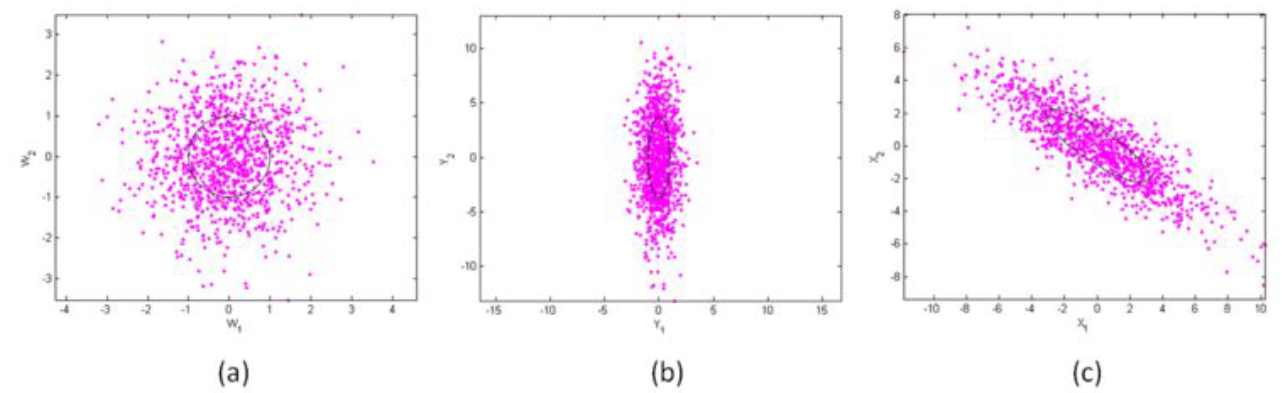
\includegraphics[width=\linewidth]{coloring.png}
	\caption{Data coloring}
	\end{subfigure}
	\caption{Whitening-Coloring-Transformation}
	\label{fig:WCT}
\end{figure}
%%%%% 3.2 stylization %%%%%
\newline
\newline\textbf{3.2  Boost}\newline